% Options for packages loaded elsewhere
\PassOptionsToPackage{unicode}{hyperref}
\PassOptionsToPackage{hyphens}{url}
%
\documentclass[
]{article}
\usepackage{lmodern}
\usepackage{amssymb,amsmath}
\usepackage{ifxetex,ifluatex}
\ifnum 0\ifxetex 1\fi\ifluatex 1\fi=0 % if pdftex
  \usepackage[T1]{fontenc}
  \usepackage[utf8]{inputenc}
  \usepackage{textcomp} % provide euro and other symbols
\else % if luatex or xetex
  \usepackage{unicode-math}
  \defaultfontfeatures{Scale=MatchLowercase}
  \defaultfontfeatures[\rmfamily]{Ligatures=TeX,Scale=1}
\fi
% Use upquote if available, for straight quotes in verbatim environments
\IfFileExists{upquote.sty}{\usepackage{upquote}}{}
\IfFileExists{microtype.sty}{% use microtype if available
  \usepackage[]{microtype}
  \UseMicrotypeSet[protrusion]{basicmath} % disable protrusion for tt fonts
}{}
\makeatletter
\@ifundefined{KOMAClassName}{% if non-KOMA class
  \IfFileExists{parskip.sty}{%
    \usepackage{parskip}
  }{% else
    \setlength{\parindent}{0pt}
    \setlength{\parskip}{6pt plus 2pt minus 1pt}}
}{% if KOMA class
  \KOMAoptions{parskip=half}}
\makeatother
\usepackage{xcolor}
\IfFileExists{xurl.sty}{\usepackage{xurl}}{} % add URL line breaks if available
\IfFileExists{bookmark.sty}{\usepackage{bookmark}}{\usepackage{hyperref}}
\hypersetup{
  hidelinks,
  pdfcreator={LaTeX via pandoc}}
\urlstyle{same} % disable monospaced font for URLs
\usepackage[margin=1in]{geometry}
\usepackage{graphicx,grffile}
\makeatletter
\def\maxwidth{\ifdim\Gin@nat@width>\linewidth\linewidth\else\Gin@nat@width\fi}
\def\maxheight{\ifdim\Gin@nat@height>\textheight\textheight\else\Gin@nat@height\fi}
\makeatother
% Scale images if necessary, so that they will not overflow the page
% margins by default, and it is still possible to overwrite the defaults
% using explicit options in \includegraphics[width, height, ...]{}
\setkeys{Gin}{width=\maxwidth,height=\maxheight,keepaspectratio}
% Set default figure placement to htbp
\makeatletter
\def\fps@figure{htbp}
\makeatother
\setlength{\emergencystretch}{3em} % prevent overfull lines
\providecommand{\tightlist}{%
  \setlength{\itemsep}{0pt}\setlength{\parskip}{0pt}}
\setcounter{secnumdepth}{-\maxdimen} % remove section numbering

\author{}
\date{\vspace{-2.5em}}

\begin{document}

{
\setcounter{tocdepth}{4}
\tableofcontents
}
\hypertarget{projects}{%
\subsection{Projects}\label{projects}}

\begin{center}\rule{0.5\linewidth}{0.5pt}\end{center}

Here are in process projects.

\begin{center}\rule{0.5\linewidth}{0.5pt}\end{center}

\hypertarget{growth-mindset-intervention}{%
\subsection{Growth Mindset
Intervention}\label{growth-mindset-intervention}}

\begin{center}\rule{0.5\linewidth}{0.5pt}\end{center}

\begin{row}

\begin{col-sm-6}

\hypertarget{growth-mindset-intervention-1}{%
\paragraph{\texorpdfstring{\href{https://katjanewilson.github.io/WhartonAnalytics-MLB/}{Growth
Mindset
Intervention}}{Growth Mindset Intervention}}\label{growth-mindset-intervention-1}}

Dual Enrollment programs offer high school students the opportunity to
explore college curricula and earn college credit before graduation.
With a large number of students participating in these programs each
year in the state of Texas, researchers have the comfort of a large
sample size and the opportunity to ethically randomize interventions. We
evaluate how changes in growth mindset influence sense of belonging,
course completion, and inclination to pursue STEM fields for a large
cohort (\textasciitilde3,000 students).

\hypertarget{technical}{%
\subparagraph{Technical}\label{technical}}

Data cleaning: tidyverse Text Analysis: tidytext

\end{col-sm-6}

\begin{col-sm-6}


\includegraphics[width=800px]{images/onramps}

\end{col-sm-6}

\end{row}

\begin{center}\rule{0.5\linewidth}{0.5pt}\end{center}

\hypertarget{khan-academy-chat}{%
\subsection{Khan Academy Chat}\label{khan-academy-chat}}

\begin{center}\rule{0.5\linewidth}{0.5pt}\end{center}

\begin{row}

\begin{col-sm-6}

\hypertarget{khan-chat}{%
\paragraph{\texorpdfstring{\href{https://katjanewilson.github.io/WhartonAnalytics-MLB/}{Khan
Chat}}{Khan Chat}}\label{khan-chat}}

Overview

\hypertarget{technical-1}{%
\paragraph{Technical}\label{technical-1}}

WebScraping: BeautifulSoup
\href{https://www.crummy.com/software/BeautifulSoup/bs4/doc/}{link}

\end{col-sm-6}

\begin{col-sm-6}


\includegraphics[width=800px]{images/onramps}

\end{col-sm-6}

\end{row}

\begin{center}\rule{0.5\linewidth}{0.5pt}\end{center}

\hypertarget{philadelphia-public-schools}{%
\subsection{Philadelphia Public
Schools}\label{philadelphia-public-schools}}

\begin{center}\rule{0.5\linewidth}{0.5pt}\end{center}

\begin{row}

\begin{col-sm-6}

\hypertarget{philadelphia}{%
\paragraph{\texorpdfstring{\href{https://katjanewilson.github.io/WhartonAnalytics-MLB/}{Philadelphia}}{Philadelphia}}\label{philadelphia}}

In experiments where randomization is not feasible, propensity score
matching helps to control for confounded relationships. Analysts working
in this causal framework often run into a particular issue: sample size
affects their ability to arrive at evenly matched samples. This problem
is especially prevalent in observational studies which use
administrative data. In a project with the Philadelphia School District,
we arrive at better percent balance improvement by trimming
mis-represented groups. *data private on github \#\#\#\#\# Technical
Data cleaning: tidyverse Causal Inference: R (MatchIt)

\end{col-sm-6}

\begin{col-sm-6}


\includegraphics[width=800px]{images/philly}

\end{col-sm-6}

\end{row}

\begin{center}\rule{0.5\linewidth}{0.5pt}\end{center}

\hypertarget{covid-19-open-research}{%
\subsection{COVID-19 Open Research}\label{covid-19-open-research}}

\begin{center}\rule{0.5\linewidth}{0.5pt}\end{center}

\begin{row}

\begin{col-sm-6}

\hypertarget{covid}{%
\paragraph{\texorpdfstring{\href{https://katjanewilson.github.io/WhartonAnalytics-MLB/}{COVID}}{COVID}}\label{covid}}

Central to the debate of ethical algorithm design is a consideration of
mis-classification costs for supervised learning methods. By building in
asymmetric costs through sampling, machine learning engineers can take
heed of policy makers' desired cost-ratios. This random forest algorithm
takes asymmetric sampling into account when predicting death rates of
coronavirus patients in South Korea using the Kaggle COVID-19 Open
Research Dataset. *course project for Stat 974

\hypertarget{technical-2}{%
\paragraph{Technical}\label{technical-2}}

Data cleaning: tidyverse Random Forest: R (randomforest)

\end{col-sm-6}

\begin{col-sm-6}

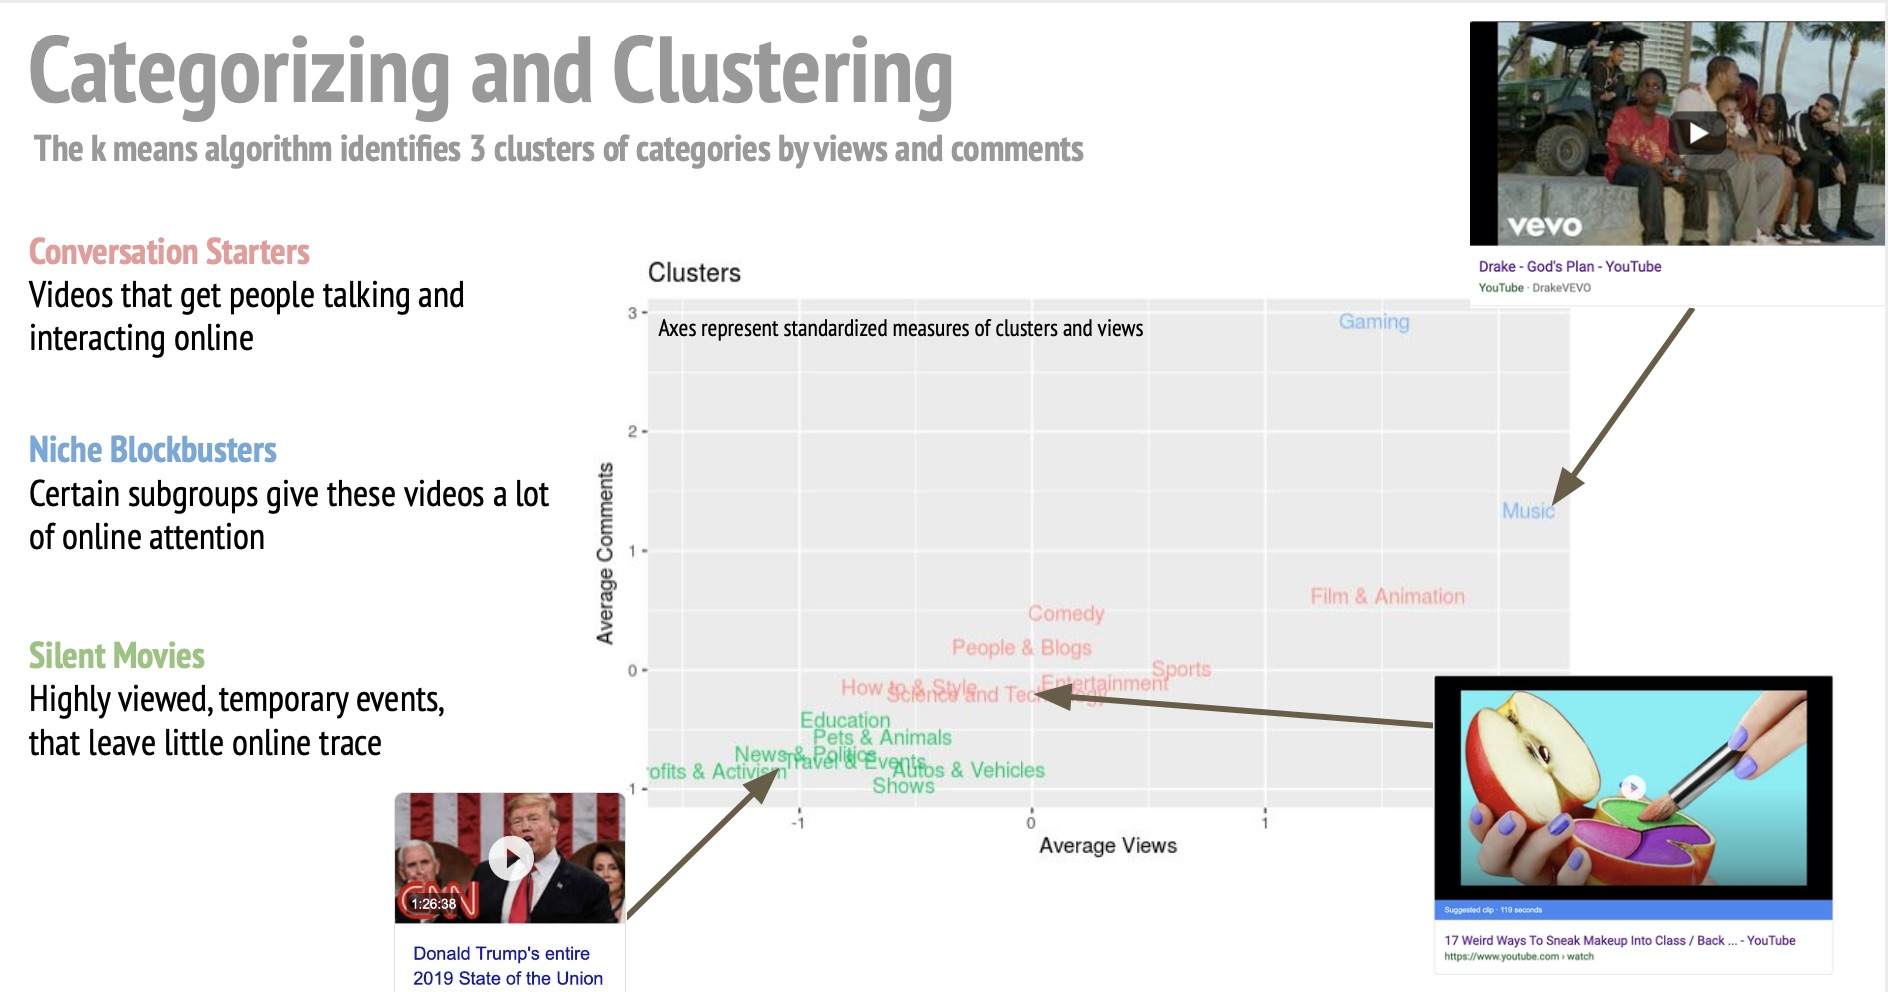
\includegraphics[width=800px]{images/image2}

\end{col-sm-6}

\end{row}

\begin{center}\rule{0.5\linewidth}{0.5pt}\end{center}

\hypertarget{los-angeles-census-tracts}{%
\subsection{Los Angeles Census Tracts}\label{los-angeles-census-tracts}}

\begin{center}\rule{0.5\linewidth}{0.5pt}\end{center}

\begin{row}

\begin{col-sm-6}

\hypertarget{la}{%
\paragraph{\texorpdfstring{\href{https://katjanewilson.github.io/WhartonAnalytics-MLB/}{LA}}{LA}}\label{la}}

A hard to swallow assumption in the linear model framework is that a
particular feature will change at the same rate across all values for a
given variable. General Additive Models (GAM) give analysts the
opportunity to identify nonlinear changes between covariates and the
dependent variable. These nonparametric models can suffer from poor
interpretability, however, and strong assumptions will have to be made
regarding the data generation process. In a project using census data in
the city of Los Angeles, GAM models identify outlier trends in homeless
individuals, yet they also reveal limitations of the loess smoother at
upper boundaries of data. *course project for Stat 974 \#\#\#\#
Technical Data cleaning: tidyverse General Additive Models: mgc, mgcViz
and gam

\end{col-sm-6}

\begin{col-sm-6}

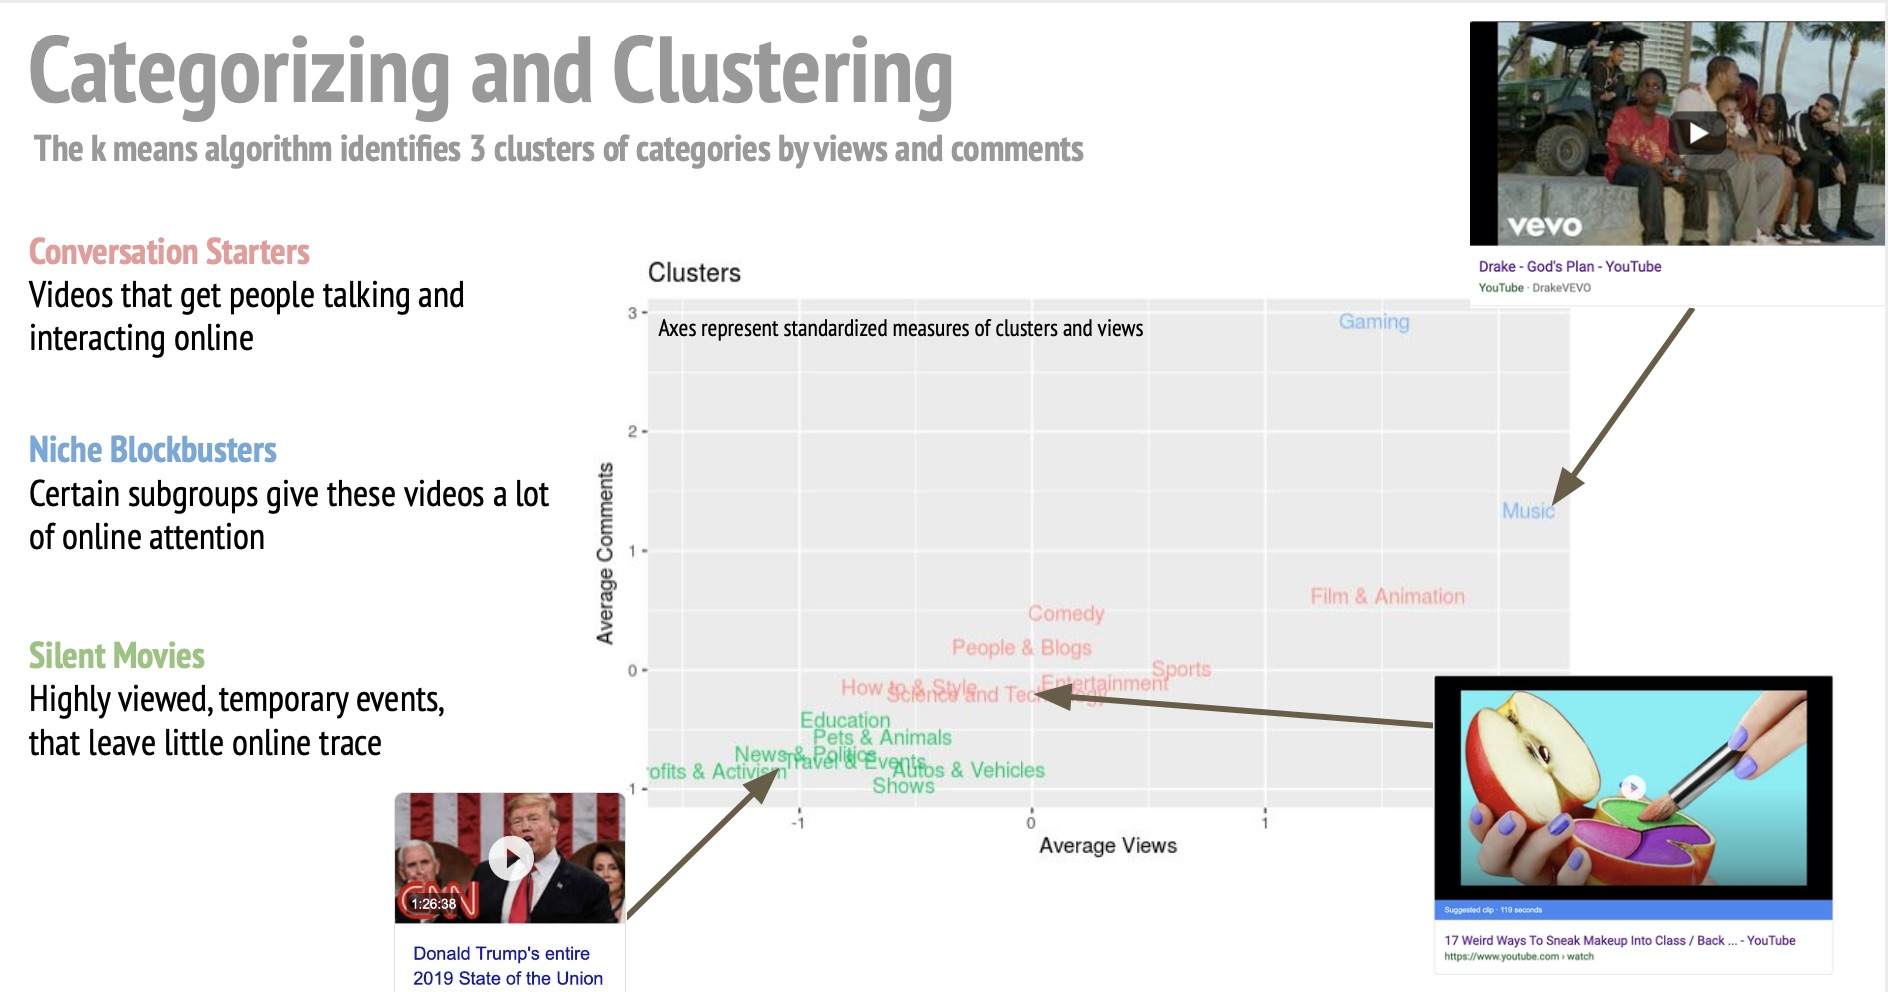
\includegraphics[width=800px]{images/image2}

\end{col-sm-6}

\end{row}

\begin{center}\rule{0.5\linewidth}{0.5pt}\end{center}

\hypertarget{spotify-web-api}{%
\subsection{Spotify Web API}\label{spotify-web-api}}

\begin{center}\rule{0.5\linewidth}{0.5pt}\end{center}

\begin{row}

\begin{col-sm-6}

\hypertarget{spot}{%
\paragraph{\texorpdfstring{\href{https://katjanewilson.github.io/WhartonAnalytics-MLB/}{Spot}}{Spot}}\label{spot}}

Data from the Spotify API are fodder for a few data journalism projects
currently in the works. One project involves visualizing changing
applause levels among an artist's studio and live recordings. With this
jitter plot, built using the JavaScript library D3.js, a user can
evaluate distances between points and visualize the ``ceiling effect''
of comparison data. \#\#\#\# Technical Web scraping: Python
(BeautifulSoup) Data Cleaning: tidyverse Data visualization: D3.js

\end{col-sm-6}

\begin{col-sm-6}

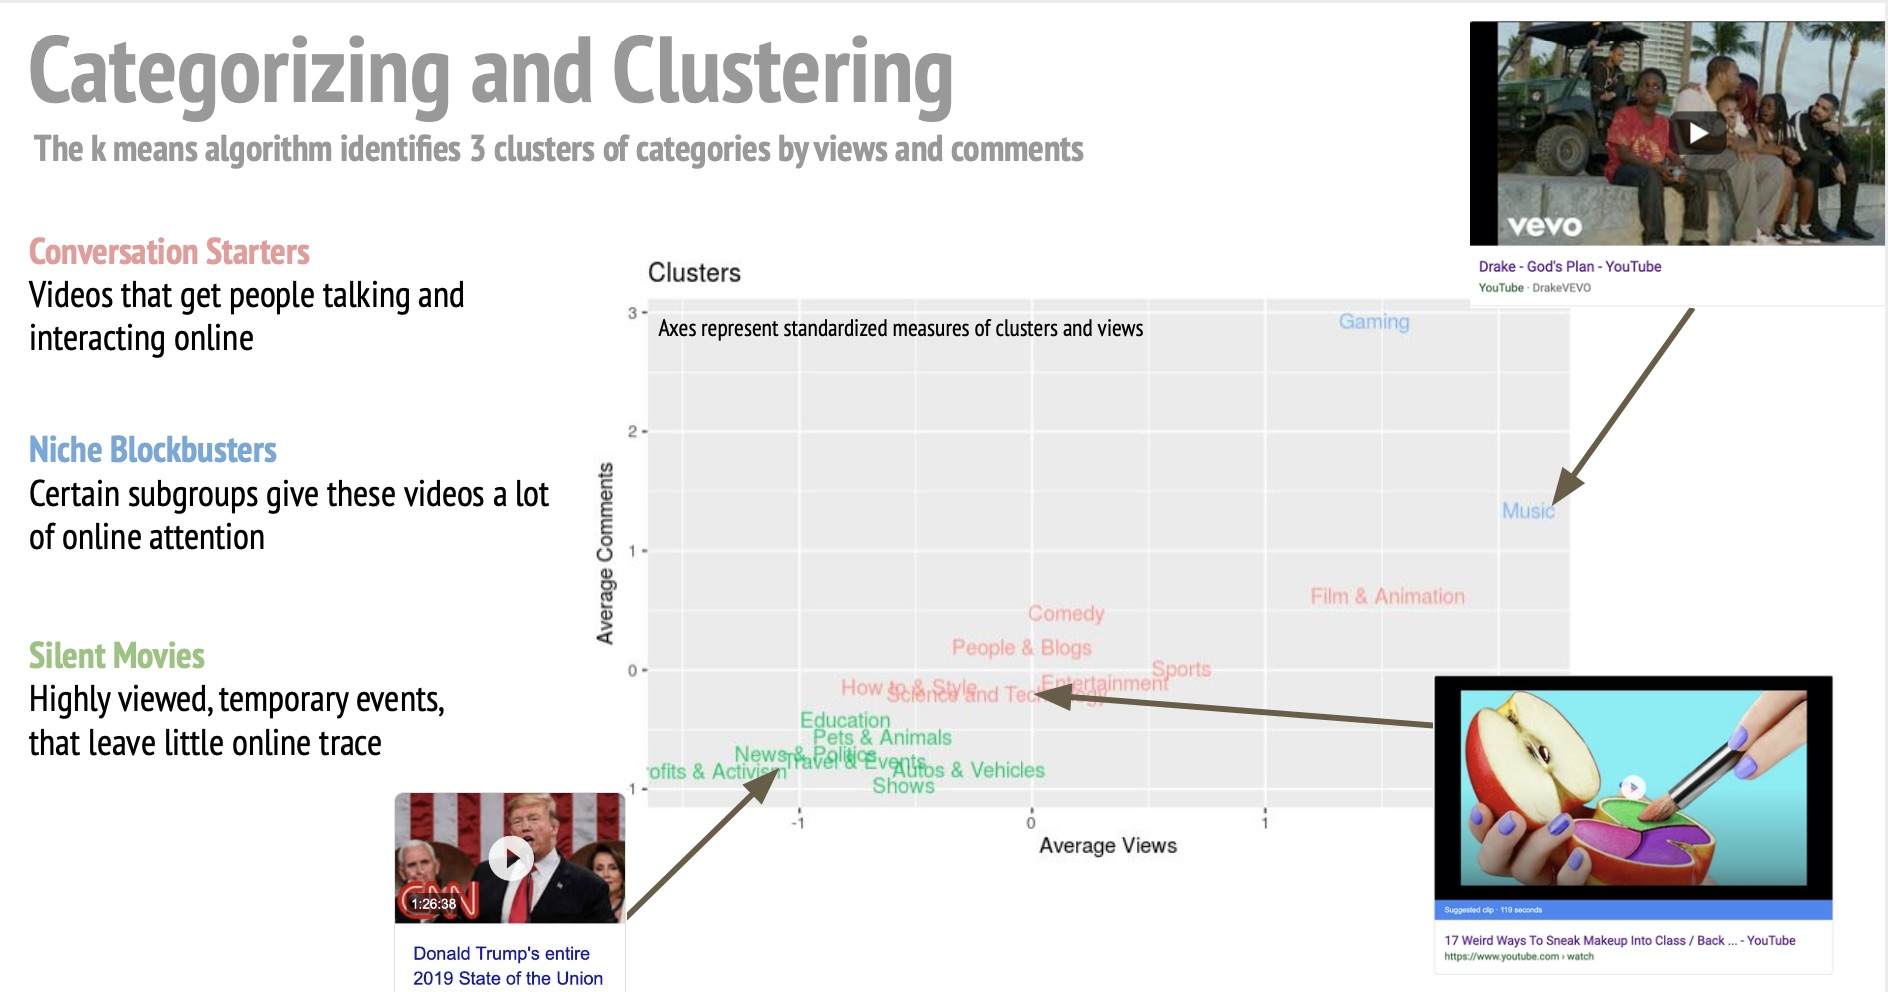
\includegraphics[width=800px]{images/image2}

\end{col-sm-6}

\end{row}

\begin{center}\rule{0.5\linewidth}{0.5pt}\end{center}

\end{document}
